\ifx\wholebook\relax \else

\documentclass{article}

\input{../common-zh-cn.tex}

\setcounter{page}{1}

\begin{document}

\title{范畴论}

\author{刘新宇
\thanks{{\bfseries 刘新宇} \newline
  Email: liuxinyu95@gmail.com \newline}
  }

\maketitle
\fi

\markboth{范畴论}{编程的数学原理}

\ifx\wholebook\relax
\chapter{范畴论}
\numberwithin{Exercise}{chapter}
\fi

\epigraph{数学是赋予不同事物相同名字的艺术。}{——昂利$\cdot$庞加莱}

% Mathematics is the art of giving the same name to different things.

\begin{wrapfigure}{R}{0.4\textwidth}
 \centering
 \includegraphics[scale=0.5]{img/dewdrop.eps}
 \captionsetup{labelformat=empty}
 \caption{艾舍尔《露珠》1948}
 \label{fig:Escher-Dewdrop-1948}
\end{wrapfigure}

如果你已经坚持看到了本书这一章,我建议你小小的奖励自己一下。你已经迈过了第一道门槛,正在通往神奇的抽象王国之路上。这条路是世界上许多最聪明的心智披荆斩棘开辟出来的。如果说,人们将具体的事物,抽象成不带具体意义的数与形是原始阶段;将数、形与计算的意义去除,抽象成代数结构(例如群)和代数关系(例如同构)是第一阶段;范畴论可以算是抽象的第二阶段。

你也许会问,我们为什么要了解范畴论?这和编程有什么关系?对此有一个比较短的答案和一个比较长的答案。较短的回答是,如果不了解范畴论,过不了多久,你也许看不懂别人写的程序了。2010年以后,如果翻看Haskell标准库的源代码,就会发现几乎所有的内容,都用范畴论重新写过了。映射、叠加、遍历……几乎所有的计算都在说着范畴的语言,犹如天书。你也许觉得叠加操作可以这样写:

\lstset{language=Haskell, frame=single}
 \begin{lstlisting}
foldr _ z [] = z
foldr f z (x:xs) = f x (foldr f z xs)
\end{lstlisting}

实际上,今天的标准库用范畴的语言这样写:

\begin{lstlisting}
foldr f z t = appEndo (foldMap (Endo #. f) t) z
foldMap f = foldr (mappend . f) mempty
\end{lstlisting}

你也许觉得,反正工作中不用Haskell,不了解范畴论也没有关系。但是最近十几年的情况是,范畴论由于其强大的抽象,几乎普适于任何问题,正向其它的语言和环境中渗透。不要说各大编程语言纷纷引入lambda演算和闭包等结构,有超过20种语言已经实现了单子\cite{Monad-Haskell-Wiki}——用范畴论的语言说,叫做“函子范畴上的幺半群”。

较长的答案是:我们需要抽象。请原谅这个答案看起来更短。赫尔曼$\cdot$外尔说现代数学在过去几十年不断沉湎在抽象和形式化上。编程领域何尝不是如此呢?现代计算机科学解决的问题空前复杂,大数据量、分布式、高并发、还要保证数据和计算的安全。仅仅靠着前几十年的传统方法——暴力求解、务实的工程实践再加上一点聪明的头脑已经不够了。这逼迫着我们去吸取其它科学和数学中的新方法和新工具。

正如迪厄多内所说:“这种抽象绝不是来自数学家的反常意愿,似乎他们想通过使用深奥莫测的语言来把自己与其它人隔开。数学家是被经典对象和关系的本质特性逼着去锻造新的抽象工具,来解决过去看来是不可攻克的问题。”\cite{Dieudonne1987}

本章内容将再次挑战我们的抽象思维。如果读完一遍没有理解是完全正常的。请不要灰心丧气,生活不是直线发展的,我们理解知识的过程是螺旋上升的。要不断回过头去反复体会。开卷有益,去阅读大师的作品。也许某个瞬间豁然开朗,就能体会到“蓦然回首,那人却在灯火阑珊处”的感觉。

范畴论是数学家艾伦伯格和麦克兰恩在1940年代创立的。

\begin{wrapfigure}{R}{0.3\textwidth}
 \centering
 \includegraphics[scale=0.25]{img/Eilenberg.eps}
 \captionsetup{labelformat=empty}
 \caption{艾伦伯格(Samuel Eilenberg, 1913 - 1998)}
 \label{fig:Eilenberg}
\end{wrapfigure}

塞缪尔·艾伦伯格于1913年生于波兰华沙的一个犹太人家庭。他于1936年在华沙大学获得博士学位。艾伦伯格主要研究代数拓扑。他与诺曼·斯廷罗德(Norman Steenrod)一起对同调理论进行了公理化。艾伦伯格在与麦克兰恩合作研究同调代数的过程中一起创立了范畴论。艾伦伯格也是著名的布尔巴基小组成员。他与昂利·嘉当合作,在1956年完成了经典著作《同调代数》。艾伦伯格后来移居美国,在纽约哥伦比亚大学做教授,他的主要工作是发展纯粹的范畴论,是该领域的奠基者之一。1986年他获得沃尔夫奖。1998年艾伦伯格逝世于美国纽约市。

艾伦伯格还是著名的亚洲艺术品收藏家。他收集了来自印度、印度尼西亚、尼泊尔、泰国、柬埔寨、斯里兰卡和中亚的雕塑和艺术品。1992年,他把自己收藏的400多件艺术品捐赠给了纽约大都会博物馆\cite{Wiki-Eilenberg}。

\begin{wrapfigure}{L}{0.3\textwidth}
 \centering
 \includegraphics[scale=1]{img/Mac-Lane.eps}
 \captionsetup{labelformat=empty}
 \caption{麦克兰恩(Saunders Mac Lane, 1909 - 2005)}
 \label{fig:Mac-Lane}
\end{wrapfigure}

桑德斯·麦克兰恩1909年生于美国康涅狄格州的诺维奇市。麦克兰恩受洗时的名字是“雷斯利·桑德斯·麦克兰恩”。但是他的父母不喜欢这个名字,所以后来就把雷斯利去掉了。麦克兰恩名字的英文本来是MacLane,他的妻子在打字时总是习惯加上一个空格变成Mac Lane,索性后来麦克兰恩就将错就错了。

麦克兰恩在高中时最喜欢化学。他的父亲在这时去世了,只好由祖父来照顾他。1926年,麦克兰恩的一个远房叔叔资助他到耶鲁学习。他的数学老师希尔带领他参加数学竞赛,并且一路过关斩将获得优胜。从此麦克兰恩下定了从事数学的决心。1930年,麦克兰恩从耶鲁毕业,获得了数学和物理学的双学位。毕业前一年,有一次在新泽西召开耶鲁橄榄球队的球迷聚会。麦克兰恩在会上被授予耶鲁优秀毕业成绩奖\cite{Wiki-Mac-Lane}。恰好芝加哥大学的新任校长哈钦斯也在这次聚会中,他鼓励麦克兰恩到芝加哥大学深造。麦克兰恩于是来到了他后来毕生工作的芝加哥大学\footnote{这里有一段小插曲,聚会后不久,哈钦斯就答应给麦克兰恩一笔奖学金。但是麦克兰恩竟然忘记申请研究生课程就直接去了芝加哥大学。当然最后他被获准入学。}。1931年他获得了硕士学位,接着获得了前往世界数学圣地——哥廷根大学进修的机会。麦克兰恩幸运的成为了最后一批前往哥廷根的美国人,不久纳粹德国就开始禁止美国人前来学习。

在哥廷根,麦克兰恩师从大数学家保罗$\cdot$伯奈斯、埃米$\cdot$诺特、赫尔曼$\cdot$外尔。在他即将获得博士学位的前夕,导师伯奈斯因为是犹太人,被纳粹政府赶出了校园,于是只好由外尔接替伯奈斯。1934年麦克兰恩获得了哥廷根数学研究所的博士学位,并返回美国\footnote{取得学位后,麦克兰恩与来自芝加哥的多罗茜$\cdot$琼斯结婚,不久后,他们夫妻一起返回了芝加哥。}。

在1944年与1945年,麦克兰恩领导了在第二次世界大战期间有卓越贡献的哥伦比亚大学应用数学小组。麦克兰恩曾任美国科学院与美国哲学会的副主席,美国数学会的主席。在领导美国数学会的期间,他提倡对现代数学教学改进的研习活动。而在1974年至1980年间,他担任了美国政府的科学顾问。1976年,以他为首的美国数学家访问团访问了中国,考察了当时中国数学学术发展。麦克兰恩于1949年获选为美国科学院院士,并在1989年获得美国国家科学奖章。

麦克兰恩的早期研究方向为域论与赋值论。1941年,麦克兰恩在访问密歇根大学时遇到了艾伦伯格。两人开始在代数和拓扑学上进行合作,并结出了累累硕果。1943年,他与艾伦伯格在研究同调代数时一起创立了范畴论。

2005年,麦克兰恩逝世于美国的旧金山。

\section{范畴}

在介绍范畴的定义前,请先暂时忘记集合、函数、映射这些概念。我们以后会看到它们在范畴论中的具体解释。

\begin{definition}
一个范畴$\pmb{C}$包括一组对象(Object)\footnote{和编程中的“面向对象”无关。这里指抽象事物。},记为$A, B, C, ...$,和一组箭头(Arrow),记为$f, g, h, ...$。它们之上定义了以下四种操作:
\begin{itemize}
\item 两个全操作\footnote{全操作(total operation)是指对于所有的对象,无一例外都存在这一操作。与之相对的是部分操作(partial operation),对于某些对象,这一操作没有定义。例如对于全体整数的集合,取相反数$x \mapsto -x$是全操作,而取倒数$x \mapsto 1/x$由于对0没有定义,所以是部分操作。},称为源(source)和目标(target)\footnote{不应把源和目标理解为名词,而应理解为动词。表示“指定源为……”,“指定目标为……”},这两个操作都将对象指定到箭头上,记为$A \arrowto{f} B$,表示箭头$f$的源是$A$,目标是$B$;
\item 第三个全操作叫恒等箭头\footnote{同样这里恒等箭头(identity arrow)应理解为动词,表示“为……指定恒等箭头”。},对于任何对象$A$,恒等箭头都指向$A$自己。记为:$A \arrowto{id_A} A$;
\item 第四个操作是一个部分操作,称为组合。它将两个箭头组合起来。如果有箭头$B \arrowto{f} C$和$A \arrowto{g} B$,则$f$和$g$的组合为$f \circ g$,读作“$g$然后$f$”。它表示$A \arrowto{f \circ g} C$。
\end{itemize}

有时我们也将箭头$A \arrowto{f} B$写成$f: A \to B$,如果上下文中对象很清楚,不会产生歧义,有时也直接简写成$f$。如果将对象简记为$Obj$,箭头简记为$Arw$,则组合操作的类型为$(\circ) : Arw \times Arw \to Arw$,表示从两个箭头产生一个新的箭头;源的类型为$src: Arw \to Obj$,表示给某一箭头指定源;目标的类型为$trg: Arw \to Obj$,表示给某一箭头指定目标;恒等箭头的类型为$id: Obj \to Arw$,表示给某一对象指定恒等箭头。

除此之外,范畴还必须满足以下两条公理:

\begin{itemize}
\item \textbf{结合性公理}:箭头组合是可结合的。对任何三个可组合的箭头$f, g, h$都有:
\[
f \circ (g \circ h) = (f \circ g) \circ h
\]
我们可以将其写为$f g h$。
\item \textbf{单位元公理}:恒等箭头对于组合运算来说相当于单位元。
对于任何箭头$A \arrowto{f} B$来说,都有:
\[
f \circ id_A = f = id_B \circ f
\]
\end{itemize}
\end{definition}

由于恒等箭头相当于单位元,我们有时也把$id_A$写成$1_A$,这样组合操作用点“$\circ$”表示,我们可以把它类比为“乘法”。下面的图有助于我们理解单位元公理:

\[
A \arrowto{id_A} A \arrowto{f} B \arrowto{id_B} B
\]

我们再看一下箭头的组合。考虑如下图的3个箭头$f, g, h$,它们组成一个三角形。

\begin{center}
\begin{tikzpicture}
  \matrix (m) [matrix of math nodes,
               row sep=3em, column sep=4em, minimum width=2em]{
     & B & \\
     A & & C \\};
  \path[-stealth]
    (m-2-1) edge node [above] {$f$} (m-1-2)
    (m-1-2) edge node [above] {$g$} (m-2-3)
    (m-2-1) edge node [below] {$h$} (m-2-3);
\end{tikzpicture}
\end{center}

可以沿着两条通路从$A$到达$C$,一条是箭头组合$g \circ f$,另一条是箭头$h$。这样我们就相当于得到了一对平行的箭头:

\begin{center}
\begin{tikzpicture}
  \matrix (m) [matrix of math nodes,
               row sep=3em, column sep=4em, minimum width=2em]{
     A & C\\};
  \path[-stealth]
    (m-1-1.north east) edge node [above] {$g \circ f$} (m-1-2.north west)
    (m-1-1.south east) edge node [below] {$h$} (m-1-2.south west);
\end{tikzpicture}
\end{center}

这两个平行的箭头可能相同,也可能不同。如果它们满足:

\[
h = g \circ f
\]

我们说这个三角形是可交换的(commute),我们后面将大量用到这个概念。

\subsection{范畴的例子}

我们需要用具体的例子来帮助理解范畴这一抽象概念。同时,前面使用的三角形图像能够帮助我们形成直观的感觉。我们会借助这种图(diagram)来对范畴及其关系进行描述。我们举的第一个例子是幺半群。回顾一下上一章中关于幺半群的定义。幺半群可以说是带有单位元的半群。而半群是二元运算满足结合律的集合。例如字符串在连接操作下构成一个幺半群,单位元是空串。

\begin{lstlisting}
instance Monoid String where
    e = ""
    (*) = (++)
\end{lstlisting}

我们可以把字符串幺半群记为$(S, \doubleplus, \texttt{""})$,不难验证它满足幺半群的条件:

\[
\begin{array}{rcl}
r \doubleplus (s \doubleplus t) = (r \doubleplus s) \doubleplus t &
\text{和} &
\texttt{""} \doubleplus s = s = s \doubleplus \texttt{""}
\end{array}
\]

我们再考虑另一个幺半群,群元素是若干个不同字符组成的集合,二元操作是集合的并,单位元是空集。记为$(C, \cup, \{\})$,将两个字符集并在一起可以获得一个更大的字符集,例如:

\[
\{a, b, c, 1, 2\} \cup \{X, Y, Z, 0, 1\} = \{a, b, c, X, Y, Z, 0, 1, 2\}
\]

我们再观察第三个幺半群,集合是包括0的自然数,二元运算是普通加法,单位元是0。记为$(N, +, 0)$。接下来我们建立这三个幺半群之间的态射(morphism),首先是从字符串幺半群$S$到字符集幺半群$C$之间的态射。任给一个字符串,我们可以把串中用到的字符组成一个字符集:

\[
S \arrowto{\phi} C \quad \quad \phi: s \mapsto \{c | c \in s\}
\]

可以验证,这个态射满足以下条件,对于任意两个字符串$r, s$,有:

\[
\begin{array}{rcl}
\phi(s \doubleplus r) = \phi(s) \cup \phi(r) & \text{和} & \phi(\texttt{""}) = \{\}
\end{array}
\]

如果我们把二元运算统一用点“$\circ$”来表示,单位元统一表示为1,则可以写成:

\[
\begin{array}{rcl}
\phi(s \circ r) = \phi(s) \circ \phi(r) & \text{和} & \phi(1) = 1
\end{array}
\]

接下来再定义从字符集$C$到自然数$N$之间的态射。任给一个字符集,我们可以将集合的大小映射为正整数,空集的大小映射为0。

\[
C \arrowto{\psi} N \quad \quad \psi: c \mapsto |c|
\]

有了这两个态射$\phi, \psi$后,我们检查一下它们的组合:

\[
S \arrowto{\phi} C \arrowto{\psi} N
\]

和

\[
S \arrowto{\psi \circ \phi} N
\]

显然组合后$\psi \circ \phi$也是一个态射。这样,我们就得到了幺半群范畴,记为$\pmb{Mon}$。其中对象是幺半群,箭头是态射。恒等箭头是从一个幺半群到它自己的态射:

\[
S \arrowto{id_R} S
\]

注意范畴$\pmb{Mon}$是包含\textbf{所有}幺半群的范畴。这是一个非常巨大的范畴。另一方面,范畴也可以很小,我们接下来看的例子只含有一个幺半群。考虑$(S, \doubleplus, \texttt{""})$,它只有一个对象,就是全体字符串的集合$S$。对于任何字符串$a$,我们都可以定义前缀映射$S \arrowto{(a \doubleplus)} S$:

\[
(a \doubleplus )(x) = a \doubleplus x
\]

这样,箭头$f = (\texttt{"hello"} \doubleplus)$,就会将字符换\texttt{"hello"}添加到任何字符串的前面,例如$f(\texttt{"Alice"})=\texttt{"helloAlice"}$。而箭头$g = (\texttt{"hi"} \doubleplus)$,它可以在任何字符串前添加前缀\texttt{"hi"}\footnote{类似地,还可以定义后缀映射$(\doubleplus b)$。例如箭头$h = (\doubleplus \texttt{"bye"})$在任何字符串后添加后缀\texttt{"bye"}。}。箭头组合$f \circ g$的含义为:

\[
\begin{array}{rl}
(f \circ g)(x) & = f(g(x)) \\
               & = \texttt{"hello"} \doubleplus (\texttt{"hi"} \doubleplus x) \\
               & = (\texttt{"hello"} \doubleplus \texttt{"hi"}) \doubleplus x) \\
               & = \texttt{"hellohi"} \doubleplus x
\end{array}
\]

表示先增加前缀\text{"hi"},然后再增加前缀\texttt{"hello"}。不难验证,任意三个这样的箭头满足结合律。接下来我们还需要检查一下单位元,也就是空串\texttt{""}。以空串作为前缀等于恒等变换:

\[
id(x) = \texttt{""} \doubleplus x = x
\]

这样我们就得到了只有一个对象的幺半群范畴,如图\ref{fig:monoid-as-category}所示。

\begin{figure}[htbp]
\centering
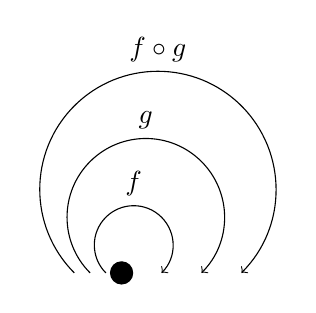
\begin{tikzpicture}
\filldraw (0, 0) circle (4pt) node (obj) {};
\draw[->] (-0.2, 0) arc[radius=5mm, start angle=225, end angle=-45] node[pos=0.5, above]{$f$};
\draw[->] (-0.4, 0) arc[radius=10mm, start angle=225, end angle=-45] node[pos=0.5, above]{$g$};
\draw[->] (-0.6, 0) arc[radius=15mm, start angle=225, end angle=-45] node[pos=0.5, above]{$f \circ g$};
\end{tikzpicture}
\caption{只有一个对象的幺半群范畴}
\label{fig:monoid-as-category}
\end{figure}

同样是幺半群,我们既看到了包含全部幺半群的范畴$\pmb{Mon}$,也看到了只包含一个幺半群的范畴。可谓一沙一世界。更有意思的是,对于任何范畴$\pmb{C}$,和其中任何的对象$a \in \pmb{C}$,定义集合$hom(a, a)$为所有从$a$指向$a$的箭头。则这一箭头的集合在组合运算下又构成一个幺半群,其中单位元是恒等箭头。这种对偶值得我们仔细体会。

类似地,群构成的范畴也有这样特点。有一个由所有群构成的巨大范畴$\pmb{Grp}$,同样每个单个的群$G$本身也构成一个范畴。前者的对象是所有的群,箭头是态射;后者只有一个对象,和幺半群比起来,群中的二元运算都有逆,所以所有的箭头都存在一个逆向的箭头。

我们举的第二个例子是集合。我们让每个集合都成为一个对象\footnote{一旦开始考虑全部集合的集合,就会对导致“全部不包括自身的集合”这样的矛盾,称之为罗素悖论。我们将在第7章详细讲述罗素悖论。},而箭头是从一个集合$A$到另一个集合$B$的函数(或映射)。我们称$A$为函数的定义域,$B$为值域\footnote{确切地说是全函数,即定义域中的每个元素都可以应用的函数}。组合运算就是函数的组合。即$y = f(x)$与$z = g(y)$的组合为$z = (g \circ f)(x) = g(f(x))$。不难验证,函数的组合满足结合律,单位元是恒等函数$id(x) = x$。这样我们就获得了全体集合和函数组成的范畴$\pmb{Set}$。

我们举的第三个例子包括一对概念。分别叫做\textbf{偏序集}和\textbf{预序集}。给定一个集合,所谓预序(pre-order),是说集合中的两个元素之间可以进行比较。我们用抽象的二元关系符号$\leq$来表示,注意这个符号不一定是大于小于关系,它可能表示一个集合是另一个集合的子集,一个字符串是另一个字符串的后缀,一个人是另一个人的后代等等。如果关系$\leq$满足以下两条性质,我们说这是一个预序关系:

\begin{itemize}
\item \textbf{自反性}:任何集合中的元素$a$都有$a \leq a$;
\item \textbf{传递性}:若$a \leq b$且$b \leq c$,则$a \leq c$;
\end{itemize}

如果在此基础上还满足反对称性,则这一关系叫做偏序(partial order):

\begin{itemize}
\item \textbf{反对称性}:若$a \leq b$且$b \leq a$,则$a = b$;
\end{itemize}

我们称满足预序关系的集合叫做预序集,满足偏序关系的集合叫做偏序集,分别记作:

\[
preset \quad \quad \quad poset
\]

\begin{figure}[htbp]
\centering
\begin{tikzpicture}[scale=0.5]
  \matrix (m) [matrix of math nodes,
               row sep=1em, column sep=1em, minimum width=2em]{
     & \text{贾演}   & & & & & \text{贾源} & & \\
     & \text{贾代化} & & & & & \text{贾代善} & & \\
     & \text{贾敬}   & & \text{贾赦} & & \text{贾政} & & & \text{贾敏} \\
     \text{贾珍} & \text{贾惜春} & \text{贾迎春} & \text{贾琏} & \text{贾珠} & \text{贾元春} & \text{贾宝玉} & \text{贾探春} & \text{贾环} \\
     \text{贾蓉} & & & \text{巧姐} & \text{贾兰} & & & & & \\};
  \path[<-]
    (m-1-2) edge (m-2-2) %贾演 -- 贾代化
    (m-1-7) edge (m-2-7) %贾源 -- 贾代善
    (m-2-2) edge (m-3-2) %贾代化 -- 贾敬
    (m-2-7) edge (m-3-4) %--贾赦
    (m-2-7) edge (m-3-6) %--贾政
    (m-2-7) edge (m-3-9) %--贾敏
    (m-3-2) edge (m-4-1) %贾敬--贾珍
    (m-3-2) edge (m-4-2) %贾敬--贾惜春
    (m-3-4) edge (m-4-3) %贾赦--贾迎春
    (m-3-4) edge (m-4-4) %贾赦--贾琏
    (m-3-6) edge (m-4-5) %贾政--贾珠
    (m-3-6) edge (m-4-6) %贾政--贾元春
    (m-3-6) edge (m-4-7) %贾政--贾宝玉
    (m-3-6) edge (m-4-8) %贾政--贾探春
    (m-3-6) edge (m-4-9) %贾政--贾环
    (m-4-1) edge (m-5-1) %贾珍--贾蓉
    (m-4-4) edge (m-5-4) %贾琏--巧姐
    (m-4-5) edge (m-5-5); %贾珠--贾兰
\end{tikzpicture}
\caption{《红楼梦》贾家的家族树}
\label{fig:genealogical-tree}
\end{figure}

在偏序集中,并非任何两个元素都能够进行比较。例如,《红楼梦》中贾家按照祖先关系构成一个偏序集。如果\ref{fig:genealogical-tree}所示。可以看到巧姐$\leq$贾琏,但是贾宝玉和贾探春之间,贾迎春和贾惜春之间无法用$\leq$进行比较。在这棵家族树中,尽管任何人都有祖先(位于树根的人根据自反性,可以认为自己是自己的祖先),但是平辈的人之间无法进行比较。不同枝干上的人之间也无法进行比较。

如图\ref{fig:powerset}所示,一个集合$\{x, y, z\}$的所有子集在包含关系下构成一个偏序集。尽管图中任意元素,都可以找到其子集,但是图中同一层级上的元素间无法比较,另外$\{x\}$和$\{y, z\}$间也无法比较。

\begin{figure}[htbp]
 \centering
 \includegraphics[scale=0.4]{img/powerset.eps}
 %\captionsetup{labelformat=empty}
 \caption{一个集合的子集在包含关系下构成一个偏序集}
 \label{fig:powerset}
\end{figure}

一般来说,任何一个偏序集都是一个预序集,但是反过来却不一定成立。一个预序集不一定是一个偏序集。考虑带有偏序(或者预序)关系的两个集合$(R, \leq)$和$(S, \leq)$。一个单调映射

\[
R \arrowto{f} S
\]

是满足如下条件的函数。对于$R$中的任意两个元素$x, y$

\[
\text{若} x \leq y \text{,则} f(x) \leq f(y)
\]

不难验证,对于任意两个单调映射:

\[
R \arrowto{f} S \arrowto{g} T
\]

它们的组合$g \circ f$也是单调映射。这样我们就获得了一对范畴

\[
\pmb{Pre} \quad \quad \quad \pmb{Pos}
\]

它们的对象分别是所有的$preset$和$poset$,两个范畴中的箭头都是单调映射。由于恒等映射也是单调映射,所以范畴中的恒等箭头为恒等映射。

考虑一对偏序集$R, S$,由于每个偏序集也是预序集,所以下面两个集合——所有从$R$出发到$S$的箭头组成的集合——是相等的。

\[
\pmb{Pre}[R, S] \quad \quad \quad \pmb{Pos}[R, S]
\]

这是因为,箭头集合中的每个元素都是一个从$R$到$S$的单调函数。这说明$\pmb{Pos}$是$\pmb{Pre}$的\textbf{子范畴}。

幺半群范畴和预序集范畴这两个例子不是随便挑选的,我们有着特殊的用意。这两个范畴可以说是最简单的例子。通过幺半群范畴,我们可以学习组合;通过预序集范畴,我们可以学习比较。对数学结构的组合与比较是整个范畴论的核心。在这一意义上,任何范畴都是幺半群与预序集的某种混合形式\cite{Simmons2011}。

$\pmb{Pre}$是包含所有预序集的巨大范畴。另一方面预序集范畴也可以很小。小到只含有一个预序集。其中的对象是预序集$(S, \leq)$中的元素$i, j, k, ...$。对于可比较的对象$i, j$,如果$i \leq j$,我们就定义箭头

\[
i \longrightarrow j
\]

这样任何对象间或者没有箭头,表示它们不可比较;或者存在一个箭头,表示它们有$\leq$关系。总之,任何两个对象间最多只有一个箭头。为了方便有时我们在箭头行做如下标记:

\[
i \arrowto{(j, i)} j
\]

看起来,似乎用$(j, i)$表示$i \leq j$像是写反了,格外别扭。实际上它会带来表达上的好处。我们来检验一下箭头的单位元和组合:

\[
\begin{array}{rll}
id_i & = (i, i) & \text{因为:} i \leq i \\
(k, j) \circ (j, i) & = (k, i) & \text{若} i \leq j \leq k \text{,则} i \leq k
\end{array}
\]

这样的确一个预序集就是一个范畴。我们再次看到了预序集范畴和幺半群范畴的对偶。幺半群作为范畴只含有一个对象,却含有丰富的箭头;预序集作为范畴对象很多,但是对象间的箭头却最多只有一个。

\begin{Exercise}
\Question{验证幺半群$(C, \cup, \{\})$和$(N, +, 0)$都是只含有一个对象的范畴。}
\Question{第一章中我们介绍了自然数的皮亚诺公理,并且介绍了和皮亚诺算术同构的其它结构,例如链表等。这些完全可以用范畴来解释。这一结论是德国数学家戴德金发现的,尽管当时还没有范畴论。我们今天将这一范畴命名为皮亚诺范畴$\pmb{Pno}$。范畴中的对象为$(A, f, z)$,其中$A$为元素的集合,对于自然数来说这个集合是全体自然数$N$;$f: A \to A$是后继函数,对于自然数来说,就是$succ$;$z \in A$是起始元素,对于自然数来说是0。任给两个皮亚诺对象$(A, f, z)$和$(B, g, c)$,现在定义态射
\[
A \arrowto{\phi} B
\]
它满足

\[
\phi \circ f = g \circ \phi \quad \text{且} \quad \phi(z) = c
\]

试验证$\pmb{Pno}$的确是一个范畴。}
\end{Exercise}

\subsection{箭头$\neq$函数}

在此前的例子中,箭头要么是一般意义上的函数,要么是类似函数意义的映射和态射。这容易造成一种错觉,认为箭头等同于函数。我们接下来看的例子有助于打破这种错觉。

\begin{example}
在这个例子中,对象是有限集合。箭头仍然是函数,但是意义变了。若集合$A$到集合$B$间有一个箭头$f$为$A \arrowto{f} B$。但是$f$的意义是这样一个函数$f: A \times B \to \mathbb{R}$,也就是说$f$接受两个自变量,分别是$A$和$B$中的元素,然后得到一个实数。如果从$B$到$C$还有一个这样的箭头$g$,其意义为:$g: B \times C \to \mathbb{R}$,则箭头的组合

\[
A \arrowto{f} B \arrowto{g} C
\]

组合的意义为:$g \circ f : A \times C \to \mathbb{R}$

这个组合函数的效果是怎样的呢?我们定义:

\[
(g \circ f)(a, c) = \sum\{f(a, x) g(x, c) | x \in B\}
\]

也就是说,我们从中间集合$B$中依次拿出每个元素$x$,计算$f(a, x)$和$g(x, c)$的积,然后将结果累加起来。显然这还是一个实数。不难验证,这构成一个范畴。
\end{example}

\begin{example}
接下来的例子名叫关系范畴$\pmb{Rel}$。范畴中的对象是集合。从对象$A$到$B$的箭头$A \arrowto{R} B$的定义为:

\[
R \subseteq B \times A
\]

我们来看看这个箭头的含义是什么。集合$B \times A$代表了所有$B$和$A$中元素对的组合。也叫做$B$和$A$的积:

\[
B \times A = \{(b, a) | a \in A, b \in B\}
\]

我们以红楼梦人物为例,集合$A =$ \{贾蓉, 贾惜春, 贾琏\},集合$B =$ \{秦可卿, 王熙凤\},则$B \times A$的积为\{(秦可卿, 贾蓉), (秦可卿, 贾惜春), (秦可卿, 贾琏), (王熙凤, 贾蓉), (王熙凤, 贾惜春), (王熙凤, 贾琏)\}。集合$R$是$B \times A$的子集,它可以看作$A$与$B$的某种关系。如果$A$中的元素$a$和$B$中的元素$b$满足关系$R$,则有$(b, a) \in R$,我们将其记为$bRa$。具体到这个例子,我们令$R=$\{(秦可卿, 贾蓉), (王熙凤, 贾琏)\},则$R$代表婚姻关系。

这样从对象$A$到$B$的\textbf{所有}箭头构成的集合$\pmb{Rel}[A, B]$就代表了从$A$到$B$的各种可能的关系。现在我们考虑箭头的组合

\[
A \arrowto{R} B \arrowto{S} C
\]

定义箭头组合$S \circ R$为:

\[
c (S \circ R) a \iff \exists b \in B \text{使得} cSbRa
\]

也就是说,存在某个中间集合中的元素$b$,同时使得两个关系$bRa$,$cSb$都成立。即$(b, a) \in R$且$(c, b) \in S$。

具体到红楼梦的例子,令集合$C=$\{王夫人, 薛姨妈, 邢夫人\},关系$S=$\{(王夫人, 王熙凤), (薛姨妈, 王熙凤)\}表示姑妈关系。这样组合箭头$S \circ R$的结果是:\{(王夫人, 贾琏), (薛姨妈, 贾琏)\},表示$c$的侄女嫁给了$b$的关系。也就是说王夫人、薛姨妈和贾琏都通过王熙凤使得两个关系同时成立。

恒等箭头的定义很简单为:

\[
id_A = \{(a, a) | a \in A\}
\]

表示所有元素都和自己产生恒等关系。
\end{example}

我们还可以从任何已知的范畴产生新的范畴,例如把一个范畴$\pmb{C}$中的所有箭头反向就得到了一个对偶的范畴$\pmb{C}^{op}$。这样我们了解了一个范畴,就同时了解了它的对偶范畴。

\begin{Exercise}
\Question{本节第一例子中的恒等箭头是什么?}
\Question{考虑集合上的部分函数构成的范畴$\pmb{Pfn}$。对象是集合,而箭头是部分函数,从集合$A$的$B$的部分函数$A \arrowto{f} B$是说,对于$A$的子集$A'$来说$f$有定义。这个范畴中的箭头组合、单位箭头的含义是什么?}
\end{Exercise}

\subsection{左右消去}

范畴中的某些箭头具有有一些特殊的性质,我们这一节介绍一对相对偶的性质,称为左消去\footnote{也有人译为“首一”,但是这里译为消去更易理解。}(monic)和右消去\footnote{有文献将monic和epic翻译为“单态射”和“满态射”。但是这只有在集合和全函数的范畴内才成立。因此本书使用左右消去的说法。}(epic)。既然是对偶的性质,我们就用对偶的形式给出:

\begin{definition}
如果范畴中的箭头
\[
B \arrowto{m} A \quad \quad \quad A \arrowto{e} B
\]
对任意一对平行的箭头

\begin{center}
\begin{tikzpicture}
  \matrix (m) [matrix of math nodes,
               row sep=3em, column sep=4em, minimum width=2em]{
     X & B & & B & X\\};
  \path[-stealth]
    (m-1-1.north east) edge node [above] {$f$} (m-1-2.north west)
    (m-1-1.south east) edge node [below] {$g$} (m-1-2.south west)
    (m-1-4.north east) edge node [above] {$f$} (m-1-5.north west)
    (m-1-4.south east) edge node [below] {$g$} (m-1-5.south west);
\end{tikzpicture}
\end{center}

均满足如下条件:

\[
\text{若} m \circ f = m \circ g \text{,则}f = g \quad \quad \quad
\text{若} f \circ e = g \circ e \text{,则}f = g
\]

我们称$m$为可\textbf{左消去}的,$e$为可\textbf{右消去}的。
\end{definition}

左右可消去箭头有一些有趣的性质,我们以左消去为例,读者可以尝试用对偶的方式思考右消去的情形。如果两个箭头是左消去的,则它们的组合也是左消去的。

\begin{proof}
令$m: A \to B$和$n: B \to C$都是左消去的,若$(n \circ m) \circ f = (n \circ m) \circ g$,我们有

\[
\begin{array}{rll}
(n \circ m) \circ f & = (n \circ m) \circ g & \\
n \circ (m \circ f) & = n \circ (m \circ g) & \text{结合律} \\
m \circ f &= m \circ g & \text{因为$n$是左消去的} \\
f & = g & \text{因为$m$是左消去的}
\end{array}
\]
所以,组合$m \circ n$也是左消去的。
\end{proof}

\begin{Exercise}
\Question{证明右消去箭头的组合也是右消去的。}
\end{Exercise}

\section{函子}
我们说范畴论是对抽象代数结构的“二次抽象”。上一节我们看到如何把所有的集合和映射、群和态射、偏序集和单调函数等抽象成范畴。接下来的问题是,如何在这些范畴之间假设桥梁、进行比较?函子\footnote{C++语言的一些资料中,用英文functor来命名函数对象,即function object。这与范畴论中的函子完全无关。}(functor)就是用来对范畴及其内在的关系(对象和箭头)进行比较的。

在某种意义上说,函子好比是范畴之间的态射。但是它不仅把一个范畴中的对象映射为另一范畴中的对象,它还将一个范畴中的箭头映射到另一个范畴中。这一点是和普通的态射(例如群之间的态射)不同的。

\subsection{函子的定义}

\begin{definition}
两个范畴$\pmb{Src}$和$\pmb{Trg}$之间的\textbf{函子}
\[
\begin{array}{rcl}
\pmb{Src} & \longrightarrow & \pmb{Trg} \\
A & \longmapsto & \mathbf{F}A \\
f & \longmapsto & \mathbf{F}(f)
\end{array}
\]
包含两部分:它将范畴$\pmb{Src}$中的对象对应到另一个范畴$\pmb{Trg}$中;并且将$\pmb{Src}$中的箭头也对应到另一个范畴$\pmb{Trg}$中。
\end{definition}

通常我们用同一个符号$\mathbf{F}$既表示对象间的变换,也表示箭头间的变换。这是一个非斜体的粗体大写字母,请注意它和范畴(粗斜体大写)、对象(斜体大写)所用字体的差别。有些编程环境,如Haskell,使用不同的记号来表示函子中对象的变换和箭头的变换。我们稍后在例子中会看到这些不同点。

既然说函子好比是范畴间的态射,那么函子必须能够忠实保持范畴间的结构和关系,这是如何做到的呢?为此函子必须满足两条性质。

\begin{itemize}
\item 第一条性质,是函子必须保持恒等箭头仍然变换为恒等箭头。用图来表示就是:

\[
A \arrowto{id_A} A \quad \longmapsto \quad \mathbf{F}A \arrowto{id_{\mathbf{F}A}} \mathbf{F}A
\]

写成公式为:

\[
\mathbf{F}(id_A) = id_{\mathbf{F}A}
\]

\item 第二条性质看似简单,实则不然。函子必须能够保持箭头的组合仍然变换为将头的组合。之所以说不简单,是因为存在两种箭头的变换方式:

\[
\begin{array}{rcll}
A \arrowto{f} B & \longmapsto & \mathbf{F}A \arrowto{\mathbf{F}(f)} \mathbf{F}B & \text{协变} \\
A \arrowto{f} B & \longmapsto & \mathbf{F}B \arrowto{\mathbf{F}(f)} \mathbf{F}A & \text{反变} \\
\end{array}
\]

其中箭头方向不变的方式叫做\textbf{协变}(covariant),而箭头方向反向的方式叫做\textbf{反变}(contravariant)。一个函子要么是协变的要么是反变的。它是一致的,因而不会对某个箭头$f$进行协变,而对另一个将头$g$进行反变。

因此对于协变函子来说,箭头的组合性质是按照下图保持的:

\begin{center}
\begin{tikzpicture}
  \matrix (m) [matrix of math nodes,
               row sep=2em, column sep=2.5em, minimum width=2em]{
       & B &   & \longmapsto &             & \mathbf{F}B & \\
     A &   & C & \text{协变} & \mathbf{F}A &  & \mathbf{F}C\\};
  \path[-stealth]
    (m-2-1) edge node [above] {$f$} (m-1-2)
    (m-1-2) edge node [above] {$g$} (m-2-3)
    (m-2-1) edge node [below] {$g \circ f$} (m-2-3)
    (m-2-5) edge node [above] {$\mathbf{F}(f)$} (m-1-6)
    (m-1-6) edge node [above] {$\mathbf{F}(g)$} (m-2-7)
    (m-2-5) edge node [below] {$\mathbf{F}(g \circ f)$} (m-2-7);
\end{tikzpicture}
\end{center}

写成公式为:

\[
\mathbf{F}(g \circ f) = \mathbf{F}(g) \circ \mathbf{F}(f)
\]

与此对应,反变函子的箭头组合性质中,箭头的方向全部反向:

\begin{center}
\begin{tikzpicture}
  \matrix (m) [matrix of math nodes,
               row sep=2em, column sep=2.5em, minimum width=2em]{
       & B &   & \longmapsto &             & \mathbf{F}B & \\
     A &   & C & \text{反变} & \mathbf{F}A &  & \mathbf{F}C\\};
  \path[-stealth]
    (m-2-1) edge node [above] {$f$} (m-1-2)
    (m-1-2) edge node [above] {$g$} (m-2-3)
    (m-2-1) edge node [below] {$g \circ f$} (m-2-3)
    (m-1-6) edge node [above] {$\mathbf{F}(f)$} (m-2-5)
    (m-2-7) edge node [above] {$\mathbf{F}(g)$} (m-1-6)
    (m-2-7) edge node [below] {$\mathbf{F}(g \circ f)$} (m-2-5);
\end{tikzpicture}
\end{center}

写成公式为:

\[
\mathbf{F}(g \circ f) = \mathbf{F}(f) \circ \mathbf{F}(g)
\]

大多数情况下,我们关注协变函子。
\end{itemize}

函子之间也可以进行组合,例如函子$(\mathbf{F} \mathbf{G})(f)$表示先用函子$\mathbf{G}$对箭头$f$进行变换,然后再用$\mathbf{F}$对这一新范畴中的箭头进行变换。习惯上我们认为函子是右结合的,所以$\mathbf{F}\mathbf{G}A$表示先对对象$A$应用函子$\mathbf{G}$,然后再应用函子$\mathbf{F}$。

\subsection{函子的例子}

\begin{wrapfigure}{R}{0.3\textwidth}
 \centering
 \includegraphics[scale=0.3]{img/blackhole.eps}
 \captionsetup{labelformat=empty}
 \caption{常数函子的行为像一个黑洞}
 \label{fig:blackhole}
\end{wrapfigure}

让我们用具体的例子来更好地理解函子的概念。我们在这一节将举一些编程中的实例。如果一个函子从一个范畴映射到这个范畴本身上,这样的函子被称为\textbf{自函子}(endo-functor)\footnote{这和代数中的自同构概念很类似。如果记不清了,请回顾一下上一章。}。最简单的函子称为“恒等函子”,它是一个自函子,记为$id: \pmb{C} \to \pmb{C}$。它可以作用到任何范畴上,将对象$A$映射为对象$A$,将箭头$f$映射为箭头$f$。

其次简单的函子叫做“常函子”,它的行为像一个黑洞,我们可以把它记作$\mathbf{K}_B : \pmb{C} \to \pmb{B}$。它可以作用到任何范畴上,把所有的对象都映射为黑洞中的对象$B$,把所有的箭头都映射为黑洞中的恒等箭头$id_B$。黑洞范畴中只有一个恒等箭头,它显然也满足箭头组合的性质:$id_B \circ id_B = id_B$。

\begin{example}
我们接下来举的例子叫做“可能函子”(maybe functor)。计算机科学家,快速排序算法的提出者,1980年图灵奖得主霍尔曾说过一段有趣的话\footnote{2009年在伦敦举行的QCon会议上}。

%\begin{wrapfigure}{L}{0.25\textwidth}
\begin{figure}[h!]
 \centering
 \includegraphics[scale=1]{img/Hoare.eps}
 \captionsetup{labelformat=empty}
 \caption{霍尔}
 \label{fig:Hoare}
\end{figure}
%\end{wrapfigure}

“我在1965年发明了空引用(null reference)。这是一个导致数十亿美元损失的发明。当时,我在为一种面向对象语言(ALGOL W)设计最早的类型系统。我希望能够保证所有的引用,经过编译器的自动检查,都是绝对安全的。但是我无法抗拒空引用的想法,它太容易实现了。此后,空引用导致了无数的错误、漏洞和系统崩溃。在过去的40年,由此导致的痛苦损失估计高达数十亿美元。”\cite{Wiki-Hoare}

% I call it my billion-dollar mistake. It was the invention of the null reference in 1965. At that time, I was designing the first comprehensive type system for references in an object oriented language (ALGOL W). My goal was to ensure that all use of references should be absolutely safe, with checking performed automatically by the compiler. But I couldn't resist the temptation to put in a null reference, simply because it was so easy to implement. This has led to innumerable errors, vulnerabilities, and system crashes, which have probably caused a billion dollars of pain and damage in the last forty years.

2015年后主流的编程环境都纷纷将Maybe概念引入以取代null来获取更安全的方法\footnote{例如Java和C++中的\texttt{Optional<T>}。}。

下图描述了$\mathbf{Maybe}$函子的行为。

\begin{center}
\begin{tikzpicture}
  \matrix (m) [matrix of math nodes,
               row sep=2em, column sep=2.5em, minimum width=2em]{
     A & \mathbf{Maybe} A \\
     B & \mathbf{Maybe} B \\};
  \path[-stealth]
    (m-1-1) edge (m-1-2)
    (m-2-1) edge (m-2-2)
    (m-1-1) edge node [left] {$f$} (m-2-1)
    (m-1-2) edge node [right] {$\mathbf{Maybe}(f)$} (m-2-2);
\end{tikzpicture}
\end{center}

图中左侧的对象$A, B$是一些数据类型,比如整形,布尔型。而右侧的对象,是通过函子$\mathbf{Maybe}$映射成的类型。如果$A$代表\texttt{Int},则右侧对应是\texttt{Maybe Int},$B$如果代表\texttt{Bool},则右侧对应的是\texttt{Maybe Bool}。可能函子是怎样完成对象的映射呢?它的对象映射部分是这样定义的:

\lstset{frame=none}
\begin{lstlisting}
data Maybe A = Nothing | Just A
\end{lstlisting}

也就是说,若对象是类型$A$,则映射到的对象是类型$\mathbf{Maybe}A$。注意,这里的对象是类型,而不是值。而类型$\mathbf{Maybe}A$的值要么是一个空值\texttt{Nothing},要么是一个用\texttt{Just}构造的值。

例如,对象是类型\texttt{Int},可能函子映射后对象是类型\texttt{Maybe Int},它的值可能是\texttt{Nothing}或者\texttt{Just 5}。

例如有一个元素类型为$A$的二叉搜索树,在其中搜索一个值时,可能会搜不到。所以搜索的结果类型是$\mathbf{Maybe}A$\footnote{完整的代码见本章附录}。

\[
\begin{array}{rcl}
lookup\ nil\ \_ & = & Nothing \\
lookup\ (Node\ l\ k\ r)\ x & = & \begin{cases}
  x < k: & lookup\ l\ x \\
  x > k: & lookup\ r\ x \\
  x = k: & Just\ k
\end{cases}
\end{array}
\]

在处理$\mathbf{Maybe}$数据类型时,必须处理可能的两种值,例如:

\[
\begin{array}{rcl}
elem\ Nothing & = & False \\
elem\ (Just\ x) & = & True
\end{array}
\]

函子既映射对象,也映射箭头。以上我们看到了$\mathbf{Maybe}$如何映射对象,那么它是如何映射箭头的呢?上面图中的左侧从上到下有一个箭头$A \arrowto{f} B$,而右侧也有一个箭头$\mathbf{Maybe}A \arrowto{\mathbf{Maybe}(f)} \mathbf{Maybe}B$。我们不妨把右侧的箭头叫做$f'$。假设我们知道左侧箭头$f$的行为,那么右侧箭头的行为是什么呢?我们说过处理$\mathbf{Maybe}$类型的数据,必须处理两种可能的值,所以$f'$的行为应该是这样的:

\[
\begin{array}{rcl}
f'\ Nothing & = & Nothing \\
f'\ (Just\ x) & = & Just\ (f\ x)
\end{array}
\]

这种给定$f$,映射成$f'$的行为恰好就是$\mathbf{Maybe}$函子对箭头进行的映射。实际的编程环境中,通常使用$fmap$来定义函子对箭头的映射。我们可以定义所有函子$\mathbf{F}$满足:

\[
fmap : (A \to B) \to (\mathbf{F} A \to \mathbf{F} B)
\]

也就是说,如果$\mathbf{F}$是一个函子,它把从$A$到$B$的箭头映射成从$\mathbf{F} A$到$\mathbf{F} B$的箭头。因此对于$\mathbf{Maybe}$函子,相应的$fmap$定义如下:

\[
\begin{array}{l}
\quad    fmap : (A \to B) \to (\mathbf{Maybe} A \to \mathbf{Maybe} B) \\
\quad    fmap\ \_\ Nothing = Nothing \\
\quad    fmap\ f\ (Just\ x) = Just\ (f\ x) \\
\end{array}
\]

回到前面二叉搜索树的例子,假如树中元素的类型是自然数,我们在树中搜索一个值,如果搜到,就将这个值转换成二进制,否则返回$Nothing$。如果我们以前已经写过一个将十进制自然数转换成二进制的函数:

\[
binary(n) = \begin{cases}
n < 2: & [n] \\
\text{否则}: & binary(\lfloor\dfrac{n}{2}\rfloor)\doubleplus[n \bmod 2]
\end{cases}
\]

下面是一个相应的Haskell代码实现。为了提高性能,这个实现使用了尾递归。

\lstset{frame=single}
\begin{lstlisting}[style=Haskell]
binary = bin [] where
   bin xs 0 = 0 : xs
   bin xs 1 = 1 : xs
   bin xs n = bin ((n `mod` 2) : xs) (n `div` 2)
\end{lstlisting}

有了函子,就可以直接将这个函数箭头“举”到上面去,如下图所示:

\begin{center}
\begin{tikzpicture}
  \matrix (m) [matrix of math nodes,
               row sep=2em, column sep=6em, minimum width=2em]{
     \mathbf{Maybe} Int & \mathbf{Maybe} [Int] \\
     Int & \left [ Int \right] \\};
  \path[-stealth]
    (m-1-1) edge node [above] {$fmap\ binary$} (m-1-2)
    (m-2-1) edge node [below] {$binary$} (m-2-2)
    (m-2-1) edge (m-1-1)
    (m-2-2) edge (m-1-2);
\end{tikzpicture}
\end{center}

这样,我们就可以直接利用Maybe函子和$binary$箭头操作二叉树搜索的结果:

\[
fmap\ binary\ (lookup\ t\ x)
\]

\begin{proof}
为了验证Maybe确是一个函子,我们还需要验证箭头映射的两条性质:

\[
\begin{array}{l}
fmap\ id = id \\
fmap\ (f \circ g) = fmap\ f \circ fmap\ g
\end{array}
\]

首先验证第一条性质。$id$的定义为:
\[
id\ x = x
\]

因此:

\[
\begin{array}{rcll}
fmap\ id\ Nothing & = & Nothing & \text{$fmap$的定义} \\
                  & = & id\ Nothing & \text{反向用$id$的定义} \\
\end{array}
\]

并且

\[
\begin{array}{rcll}
fmap\ id\ (Just\ x) & = & Just\ (id\ x) & \text{$fmap$的定义} \\
                    & = & Just\ x & \text{$id$的定义} \\
                    & = & id\ (Just\ x) & \text{反向用$id$的定义}
\end{array}
\]

接下来验证第二条性质:

\[
\begin{array}{rcll}
fmap\ (f \circ g)\ Nothing & = & Nothing & \text{$fmap$的定义} \\
           & = & fmap\ f\ Nothing & \text{反向使用$fmap$的定义} \\
           & = & fmap\ f\ (fmap\ g\ Nothing) & \text{反向使用$fmap$的定义} \\
           & = & (fmap\ f\ \circ fmap\ g)\ Nothing & \text{反向用函数组合的定义}
\end{array}
\]

并且

\[
\begin{array}{rcll}
fmap\ (f \circ g)\ (Just\ x) & = & Just\ ((f \circ g)\ x) & \text{$fmap$的定义} \\
           & = & Just\ (f\ (g\ x)) & \text{函数组合的定义} \\
           & = & fmap\ f\ (Just\ (g\ x)) & \text{反向使用$fmap$的定义} \\
           & = & fmap\ f\ (fmap\ g\ (Just\ x)) & \text{反向使用$fmap$的定义} \\
           & = & (fmap\ f\ \circ fmap\ g)\ (Just\ x) & \text{反向用函数组合的定义}
\end{array}
\]

因此Maybe的确是一个函子。
\end{proof}
\end{example}

\begin{example}
接下来介绍的例子是列表函子。第一章中我们介绍了列表的定义:

\lstset{frame=none}
\begin{lstlisting}
data List A = nil | cons(A, List A)
\end{lstlisting}

从编程的观点看,这定义了“单向链表”的数据结构,链表中元素的类型是$A$,这样的链表称为类型为$A$的列表。从范畴的观点来看,一个列表函子要分别定义对象和箭头的映射。在这里,对象是类型,箭头是全函数。下图描述了列表函子的行为:

\begin{center}
\begin{tikzpicture}
  \matrix (m) [matrix of math nodes,
               row sep=2em, column sep=2.5em, minimum width=2em]{
     A & \mathbf{List}\ A \\
     B & \mathbf{List}\ B \\};
  \path[-stealth]
    (m-1-1) edge (m-1-2)
    (m-2-1) edge (m-2-2)
    (m-1-1) edge node [left] {$f$} (m-2-1)
    (m-1-2) edge node [right] {$\mathbf{List}(f)$} (m-2-2);
\end{tikzpicture}
\end{center}

图中左侧的对象$A, B$是数据类型,例如整型、布尔型甚至是$\mathbf{Maybe}\ Char$这样的复杂类型。而右侧的对象,是通过列表函子映射成的类型,如果$A$为整形$Int$,则右侧对应$\mathbf{List}\ Int$,如果$B$代表$Char$,则右侧对应的是$\mathbf{List}\ Char$,也就是$String$。

请再次注意这里的对象是类型,而不是值,$A$可以是$Int$,但不是具体的值5。因此$\mathbf{List}\ A$对应整形列表,是一个类型,而不是一个具体的值,如:[1, 1, 2, 3, 5]。那么如何产生具体的列表值呢?那要靠$nil$和$cons$两个具体的函数来产生空值或者$list(1, list(1, list(2, nil)))$。

以上是列表函子在对象映射时的行为,那么它是如何对箭头进行映射的呢?也就是说,给定一个函数$f: A \to B$,如何通过列表函子得到另一个函数$g: \mathbf{List}\ A \to \mathbf{List}\ B$呢?与可能函子$\mathbf{Maybe}$类似,我们可以定义一个$fmap$实现从箭头$f$到箭头$g$的映射,对于列表函子它的类型为:

\[
fmap: (A \to B) \to (\mathbf{List}\ A \to \mathbf{List}\ B)
\]

接下来需要仔细分析$g$的行为。首先考虑最简单的情况,不管箭头$f$的定义如何,如果$\mathbf{List}\ A$是个空列表$nil$,则应用$g$后的结果也必然是空列表。所以有:

\[
fmap\ \_\ nil = nil
\]

接下来考虑递归的情况$cons(x, xs)$,其中$x$是类型为$A$的某个值,而$xs$是类型为$\mathbf{List}\ A$的子列表。如果$f(x) = y$,将类型$A$的值$x$映射为类型$B$的值$y$,那么我们就将$f$应用到$x$上,然后在将其递归地应用到子列表$xs$上从而得到一个元素类型为$B$的子列表$ys$,最后再将$y$和$ys$链接起来得到最终的结果:

\[
fmap\ f\ cons(x, xs) = cons(f\ x, fmap\ f\ xs)
\]

综上,我们得到了$fmap$的完整定义:

\[
\begin{array}{l}
\quad    fmap : (A \to B) \to (\mathbf{List}\ A \to \mathbf{List}\ B) \\
\quad    fmap\ \_\ nil = nil \\
\quad    fmap\ f\ cons(x, xs) = cons(f\ x, fmap\ f\ xs) \\
\end{array}
\]

如果使用第一章介绍的简记法,用冒号“:”表示$cons$,用中括号表示列表,用“[]”表示$nil$,则列表函子的箭头部分映射可以简写为:

\[
\begin{array}{l}
\quad    fmap : (A \to B) \to (\mathbf{List}\ A \to \mathbf{List}\ B) \\
\quad    fmap\ \_\ [] = [] \\
\quad    fmap\ f\ (x:xs) = (f\ x):(fmap\ f\ xs) \\
\end{array}
\]

仔细观察这个定义,再和第一章中列表的“逐一映射”定义对比,会发现它们除了名字之外完全一样,因此我们可以复用列表的“逐一映射”来定义列表函子,例如Haskell中列表函子的定义就是通过复用\texttt{map}实现的。

\lstset{frame=single}
\begin{lstlisting}
instance Functor [] where
    fmap = map
\end{lstlisting}

作为本例的结尾,我们来验证一下列表函子的箭头映射部分是否满足组合和恒等的两条性质。即:

\[
\begin{array}{l}
fmap\ id = id \\
fmap\ (f \circ g) = fmap\ f \circ fmap\ g
\end{array}
\]

\begin{proof}
我们用数学归纳法来验证恒等性质,首先针对空列表的情况:

\[
\begin{array}{rcll}
fmap\ id\ nil & = & nil & \text{$fmap$的定义} \\
              & = & id\ nil & \text{反向用$id$的定义} \\
\end{array}
\]

针对$(x:xs)$的递归情况,令递归假设为$fmap\ id\ xs = id\ xs$,我们有:

\[
\begin{array}{rcll}
fmap\ id\ (x:xs) & = & (id\ x):(fmap\ id\ xs) & \text{$fmap$的定义} \\
                 & = & (id\ x):(id\ xs) & \text{递归假设} \\
                 & = & x:xs & \text{$id$的定义} \\
                 & = & id\ (x:xs) & \text{反向用$id$的定义}
\end{array}
\]

同样,我们用数学归纳法来验证组合性质,对于空列表,我们有:

\[
\begin{array}{rcll}
fmap\ (f \circ g)\ nil & = & nil & \text{$fmap$的定义} \\
           & = & fmap\ f\ nil & \text{反向使用$fmap$的定义} \\
           & = & fmap\ f\ (fmap\ g\ nil) & \text{反向使用$fmap$的定义} \\
           & = & (fmap\ f\ \circ fmap\ g)\ nil & \text{反向用函数组合的定义}
\end{array}
\]

针对$(x:xs)$的递归情况,令递归假设为$fmap\ (f \circ g)\ xs = (fmap\ f \circ fmap\ g)\ xs$,我们有:

\[
\begin{array}{rcll}
fmap\ (f \circ g)\ (x:xs) & = & ((f \circ g)\ x):(fmap\ (f \circ g)\ xs) & \text{$fmap$的定义} \\
  & = & ((f \circ g)\ x):((fmap\ f \circ fmap\ g)\ xs) & \text{递归假设} \\
  & = & (f(g\ x)):(fmap\ f\ (fmap\ g\ xs)) & \text{函数组合的定义} \\
  & = & fmap\ f\ ((g\ x):(fmap\ g\ xs)) & \text{反向使用$fmap$的定义} \\
  & = & fmap\ f\ (fmap\ g\ (x:xs)) & \text{再次反向使用$fmap$的定义} \\
  & = & (fmap\ f\ \circ fmap\ g)\ (x:xs) & \text{反向用函数组合的定义}
\end{array}
\]

这就验证了$\mathbf{List}$的确是一个函子。
\end{proof}
\end{example}

\begin{Exercise}
\Question{请使用叠加操作$foldr$来定义列表函子的箭头映射。}
\Question{证明可能函子和列表函子的组合$\mathbf{Maybe} \circ \mathbf{List}$与$\mathbf{List} \circ \mathbf{Maybe}$仍然是函子。}
\Question{证明任意函子的组合$\mathbf{G} \circ \mathbf{F}$仍然是函子。}
\Question{思考一个预序集范畴上的函子的例子。}
\Question{回顾第二章中介绍的二叉树,请定义一个二叉树函子。}
\end{Exercise}

\section{积和余积}

在介绍更复杂的范畴和函子的例子之前,我们先了解一下积和余积的概念。这里的积是指范畴的积。为了容易理解,我们先从集合的积入手。两个集合$A$和$B$的笛卡尔积$A \times B$,是所有有序对$(a, b)$的集合。其中$a \in A, b \in B$。即:

\[
\{(a, b) | a \in A, b \in B\}
\]

例如有限集合$\{1, 2, 3\}$和$\{a, b\}$的积为

\[
\{(1, a), (2, a), (3, a), (1, b), (2, b), (3, b)\}
\]

如果集合$A, B$是同类的代数结构,如群、环等,我们可以定义如下图的对象和箭头。

\begin{center}
\begin{tikzpicture}
  \matrix (m) [matrix of math nodes,
               row sep=2em, column sep=2em, minimum width=2em]{
      &   & (a, b) &  & \\
      &   & A \times B & & \\
      &   &            & & \\
    a & A &            & B & b \\};
  \path[|->]
    (m-1-3) edge (m-4-1)
    (m-1-3) edge (m-4-5);
  \path[-stealth]
    (m-2-3) edge (m-4-2)
    (m-2-3) edge (m-4-4);
\end{tikzpicture}
\end{center}

还有一种对偶的构造,我们可以从两个集合$A, B$产生一个不相交的并集(disjoint union,也称为和)$A + B$。为了分清和中的每个元素究竟是来自$A$还是$B$,可以给元素增加一个标记(tag):

\[
A + B = (A \times \{0\}) \cup (B \times \{1\})
\]

或者等价地这样定义:

\[
A + B = zip\ A\ \{0, ...\} \doubleplus zip\ B\ \{1, ...\}
\]

当从$A+B$中取出一个元素$(x, tag)$,如果$tag$为0,我们就知道$x$本来属于$A$,如果$tag$为1,就知道$x$本来属于$B$。这样有限集合$\{1, 2, 3\}$和$\{a, b\}$的和就是

\[
\{(1, 0), (2, 0), (3, 0), (a, 1), (b, 1)\}
\]

当$A, B$是同类的代数结构时,我们可以定义如下的对象和箭头:

\begin{center}
\begin{tikzpicture}
  \matrix (m) [matrix of math nodes,
               row sep=2em, column sep=2em, minimum width=2em]{
    a & A &        &       &        & B & b \\
      &   &        &       &        &   & \\
      &   & (a, 0) & A + B & (b, 1) &   & \\};
  \path[|->]
    (m-1-1) edge (m-3-3)
    (m-1-7) edge (m-3-5);
  \path[-stealth]
    (m-1-2) edge (m-3-4)
    (m-1-6) edge (m-3-4);
\end{tikzpicture}
\end{center}

对比这两种构造我们发现它们是对偶的。如果把两张图旋转90度,把$A$画在上面,$B$画在下面,这样两个问题一个在左侧,一个在右侧。如同双手一样对称。

\subsection{积和余积的定义}

\begin{definition}
对于范畴$\pmb{C}$中的一对对象$A$和$B$,一个

\[
\text{指向$A, B$的} \quad \quad \quad \text{从$A, B$出发的}
\]

\textbf{楔形}(wedge)是范畴$\pmb{C}$中的一个对象$X$和一对箭头:

\begin{center}
\begin{tikzpicture}
  \matrix (m) [matrix of math nodes,
               row sep=2em, column sep=2em, minimum width=2em]{
      & A &  & A & \\
    X &   &  &   & X \\
      & B &  & B & \\};
  \path[-stealth]
    (m-2-1) edge (m-1-2)
    (m-2-1) edge (m-3-2)
    (m-1-4) edge (m-2-5)
    (m-3-4) edge (m-2-5);
\end{tikzpicture}
\end{center}
\end{definition}

给定范畴中的一对对象$A$和$B$,可能有不止一个向左的或者向右的楔形。我们关心那个“最好”的楔形,它距离两个对象“最近”。本质上,我们说在寻找一个泛性的(universal)楔形。这就引出了下面的(一对)定义:

\begin{definition}
对于范畴$\pmb{C}$中的一对对象$A$和$B$,一个

\[
\text{积(product)} \quad \quad \quad \text{余积(coproduct)}
\]

是一个特殊的楔形:

\begin{center}
\begin{tikzpicture}
  \matrix (m) [matrix of math nodes,
               row sep=2em, column sep=2em, minimum width=2em]{
      & A &  & A & \\
    S &   &  &   & S \\
      & B &  & B & \\};
  \path[-stealth]
    (m-2-1) edge node [above] {$p_A$} (m-1-2)
    (m-2-1) edge node [below] {$p_B$} (m-3-2)
    (m-1-4) edge node [above] {$i_A$} (m-2-5)
    (m-3-4) edge node [below] {$i_B$} (m-2-5);
\end{tikzpicture}
\end{center}

这个楔形满足如下泛性性质:对于任意楔形,

\begin{center}
\begin{tikzpicture}
  \matrix (m) [matrix of math nodes,
               row sep=2em, column sep=2em, minimum width=2em]{
      & A &  & A & \\
    X &   &  &   & X \\
      & B &  & B & \\};
  \path[-stealth]
    (m-2-1) edge node [above] {$f_A$} (m-1-2)
    (m-2-1) edge node [below] {$f_B$} (m-3-2)
    (m-1-4) edge node [above] {$f_A$} (m-2-5)
    (m-3-4) edge node [below] {$f_B$} (m-2-5);
\end{tikzpicture}
\end{center}

都存在一个唯一的箭头:

\[
 X \arrowto{m} S \quad \quad \quad S \arrowto{m} X
\]

使得下面图中的箭头可交换。

\begin{center}
\begin{tikzpicture}
  \matrix (m) [matrix of math nodes,
               row sep=2em, column sep=2em, minimum width=2em]{
      & A &  & A & \\
    X & S &  & S & X \\
      & B &  & B & \\};
  \path[-stealth]
    % left
    (m-2-1) edge node [above] {$f_A$} (m-1-2)
    (m-2-1) edge node [below] {$f_B$} (m-3-2)
    (m-2-1) edge node [above] {$m$}   (m-2-2)
    (m-2-2) edge node [right] {$p_A$} (m-1-2)
    (m-2-2) edge node [right] {$p_B$} (m-3-2)
    % right
    (m-1-4) edge node [above] {$f_A$} (m-2-5)
    (m-3-4) edge node [below] {$f_B$} (m-2-5)
    (m-2-4) edge node [above] {$m$}   (m-2-5)
    (m-1-4) edge node [right] {$i_A$} (m-2-4)
    (m-3-4) edge node [right] {$i_B$} (m-2-4);
\end{tikzpicture}
\end{center}

其中箭头$m$叫做楔形$X$的媒介箭头(mediating arrow或者mediator)
\end{definition}

在这一定义中,积或者余积并不仅仅是一个对象$S$,而是一个对象加上一对箭头。其次,对于任意给定的$X$,媒介箭头$m$都是唯一的。所谓箭头可交换,我们用左侧的积来举例,是说箭头间的关系满足:

\[
\begin{array}{l}
f_A = p_A \circ m \\
f_B = p_B \circ m
\end{array}
\]

这立刻告诉我们,下面的特例一定成立:如果$X$等于$S$,$m$是一个自箭头(endo-arrow)

\[
S \arrowto{m} S
\]

则$m$是恒等箭头。范畴图简化为:

\begin{center}
\begin{tikzpicture}
  \matrix (m) [matrix of math nodes,
               row sep=3em, column sep=3em, minimum width=2em]{
      & A &  & A & \\
    S & S &  & S & S \\
      & B &  & B & \\};
  \path[-stealth]
    % left
    (m-2-1) edge node [above] {$p_A$} (m-1-2)
    (m-2-1) edge node [below] {$p_B$} (m-3-2)
    (m-2-1) edge node [above] {$id_S$} (m-2-2)
    (m-2-2) edge node [right] {$p_A$} (m-1-2)
    (m-2-2) edge node [right] {$p_B$} (m-3-2)
    % right
    (m-1-4) edge node [above] {$i_A$} (m-2-5)
    (m-3-4) edge node [below] {$i_B$} (m-2-5)
    (m-2-4) edge node [above] {$id_S$} (m-2-5)
    (m-1-4) edge node [right] {$i_A$} (m-2-4)
    (m-3-4) edge node [right] {$i_B$} (m-2-4);
\end{tikzpicture}
\end{center}

这一结论自然会引入下面的问题:在众多的楔形中,积和余积是特殊的——它们是泛性的,是“最接近”或者说是“最好”的一个楔形。那么积和余积是唯一的么?下面的定理回答了这个问题:

\begin{lemma}
对于范畴$\pmb{C}$中的一对对象$A$和$B$,令下图中的对象和箭头

\begin{center}
\begin{tikzpicture}
  \matrix (m) [matrix of math nodes,
               row sep=2em, column sep=2em, minimum width=2em]{
    P &   &  &   & I \\
      & A &  & A &   \\
      & B &  & B &   \\
    Q &   &  &   & J \\};
  \path[-stealth]
    % left
    (m-1-1) edge node [above] {$p_A$} (m-2-2)
    (m-1-1) edge node [below] {$p_B$} (m-3-2)
    (m-4-1) edge node [above] {$q_A$} (m-2-2)
    (m-4-1) edge node [below] {$q_B$} (m-3-2)
    % right
    (m-2-4) edge node [above] {$i_A$} (m-1-5)
    (m-2-4) edge node [above] {$j_A$} (m-4-5)
    (m-3-4) edge node [below] {$i_B$} (m-1-5)
    (m-3-4) edge node [below] {$j_B$} (m-4-5);
\end{tikzpicture}
\end{center}

各自为一对

\begin{center}
积 \quad \quad \quad 余积
\end{center}

的楔形。则

\[
P, Q \quad \quad \quad I, J
\]

是同构的楔形,存在唯一的箭头:

\begin{center}
\begin{tikzpicture}
  \matrix (m) [matrix of math nodes,
               row sep=2em, column sep=3em, minimum width=2em]{
    P & & I \\
    Q & & J \\};
  \path[-stealth]
    % left
    (m-1-1.south west) edge node [left] {$f$} (m-2-1.north west)
    (m-2-1.north east) edge node [right] {$g$} (m-1-1.south east)
    % right
    (m-1-3.south west) edge node [left] {$f$} (m-2-3.north west)
    (m-2-3.north east) edge node [right] {$g$} (m-1-3.south east);
\end{tikzpicture}
\end{center}

使得:

\[
\begin{array}{lcl}
  \begin{cases}
    p_A = q_A \circ f & p_B = q_B \circ f \\
    q_A = p_A \circ g & q_B = p_B \circ g
  \end{cases}
  & \quad &
  \begin{cases}
    i_A = g \circ j_A & i_B = g \circ j_B \\
    j_A = f \circ i_A & j_B = f \circ i_B
  \end{cases}
\end{array}
\]

并且,$f$和$g$是互逆的同构箭头对。
\end{lemma}

\begin{proof}
我们只证明左侧积的部分,右侧余积部分的证明与此类似。给定$A, B$,对象$Q$和两个箭头$q_A, q_B$构成的楔形是一个积。我们把对象$P$和一对箭头$p_A, p_B$看成是另一个楔形。根据积的定义,存在唯一的媒介箭头$f$满足:

\[
p_A = q_A \circ f \quad \text{和} \quad p_B = q_B \circ f
\]

交换$P$和$Q$(另$P$为积,$Q$为任意楔形),又可以得到:

\[
q_A = p_A \circ g \quad \text{和} \quad q_B = p_B \circ g
\]

这样就有:

\[
\begin{array}{l}
p_A \circ g \circ f = q_A \circ f = p_A \\
p_B \circ g \circ f = q_B \circ f = p_B
\end{array}
\]

因此:

\[
g \circ f = id_P \quad \quad \quad f \circ g = id_Q
\]

\end{proof}

这一结论说明,如果两个对象存在积(或者余积)则它是唯一的。但是积和余积并不总是同时存在,甚至有可能都不存在。现在我们回过头来再看一下集合的情形。

\begin{lemma}
若$A, B$是两个集合,则它们的

\begin{center}
笛卡尔积$A \times B$ \quad \quad \quad 不相交并集$A + B$
\end{center}

在范畴$\pmb{Set}$中构成

\begin{center}
积 \quad \quad \quad 余积
\end{center}
 \end{lemma}

\begin{proof}
我们可以用构造法证明。首先证明左侧积的部分。$A \times B$的笛卡尔积是来自两个集合的元素对的全部组合

\[
\{(a, b) | a \in A, b \in B\}
\]

我们定义两个特殊的箭头(函数)作为$p_A$和$p_B$

\[
\begin{cases}
fst\ (a, b) = a \\
snd\ (a, b) = b
\end{cases}
\]

考虑任意楔形

\begin{center}
\begin{tikzpicture}
  \matrix (m) [matrix of math nodes,
               row sep=2em, column sep=2em, minimum width=2em]{
      & A  \\
    X &    \\
      & B  \\};
  \path[-stealth]
    (m-2-1) edge node[above] {$p$} (m-1-2)
    (m-2-1) edge node[below] {$q$} (m-3-2);
\end{tikzpicture}
\end{center}

其中$p\ x = a, q\ x = b, x \in X$。举个具体的例子,$X$为$Int$, $A$为$Int$,$B$为$Bool$,而两个函数$p, q$的定义为:

\[
\begin{cases}
p(x) = -x \\
q(x) = even(x)
\end{cases}
\]

也就是说,$p$对一个整数取相反数,$q$判断其是否是偶数。我们定义函数$X \arrowto{m} A \times B$如下:

\[
m(x) = (a, b)
\]

具体到上面的例子,有:

\[
m(x) = (-x, even(x))
\]

这样,下面图中的箭头就可交换了:

\begin{center}
\begin{tikzpicture}
  \matrix (m) [matrix of math nodes,
               row sep=2em, column sep=2em, minimum width=2em]{
      & A \\
    X & A \times B \\
      & B \\};
  \path[-stealth]
    % left
    (m-2-1) edge node [above] {$p$} (m-1-2)
    (m-2-1) edge node [below] {$q$} (m-3-2)
    (m-2-1) edge node [above] {$m$}   (m-2-2)
    (m-2-2) edge node [right] {$fst$} (m-1-2)
    (m-2-2) edge node [right] {$snd$} (m-3-2);
\end{tikzpicture}
\end{center}

不难验证:

\[
\begin{array}{rcll}
(fst \circ m)(x) & = & fst\ m(x) & \text{函数组合} \\
                 & = & fst\ (a, b) & \text{$m$的定义} \\
                 & = & a & \text{$fst$的定义} \\
                 & = & p(x) & \text{反向用$p$的定义}
\end{array}
\]

并且:

\[
\begin{array}{rcll}
(snd \circ m)(x) & = & snd\ m(x) & \text{函数组合} \\
                 & = & snd\ (a, b) & \text{$m$的定义} \\
                 & = & b & \text{$snd$的定义} \\
                 & = & q(x) & \text{反向用$q$的定义}
\end{array}
\]

具体到上面的例子,有:

\[
\begin{cases}
(fst \circ m)(x) = fst\ (-x, even(x)) = -x = p(x) \\
(snd \circ m)(x) = snd\ (-x, even(x)) = even(x) = q(x)
\end{cases}
\]

我们还需要证明$m$是唯一的。假设存在另一个函数$x \arrowto{h} A \times B$,也使得范畴图中的箭头可交换。即:

\[
fst \circ h = p \quad \text{且} \quad snd \circ h = q
\]

我们有:

\[
\begin{array}{rcll}
(a, b) & = & (p(x),\ q(x)) & \text{$p, q$的定义} \\
       & = & ((fst \circ h)(x),\ (snd \circ h)(x)) & \text{可交换} \\
       & = & (fst\ h(x),\ snd\ h(x)) & \text{函数组合} \\
       & = & (fst\ (a, b),\ snd\ (a, b)) & \text{反向用$fst, snd$的定义}
\end{array}
\]

所以$h(x) = (a, b) = m(x)$。这样就证明了$m$的唯一性。

接下来,我们证明右侧的余积部分。不相交的并集$A+B$中的元素分为两类。一类是来自$A$中的元素$(a, 0)$,另一类是来自$B$中的元素$(b, 1)$。为此,我们定义两个特殊的箭头(函数)作为$i_A, i_B$:

\[
\begin{cases}
left(a) = (a, 0) \\
right(b) = (b, 1)
\end{cases}
\]

考虑任意集合$X$构成的楔形:

\begin{center}
\begin{tikzpicture}
  \matrix (m) [matrix of math nodes,
               row sep=2em, column sep=2em, minimum width=2em]{
    A & \\
      & X \\
    B & \\};
  \path[-stealth]
    (m-1-1) edge node [above] {$p$} (m-2-2)
    (m-3-1) edge node [below] {$q$} (m-2-2);
\end{tikzpicture}
\end{center}

我们定义箭头$A + B \arrowto{m} X$如下:

\[
\begin{cases}
m\ (a, 0) = p(a) \\
m\ (b, 1) = q(b)
\end{cases}
\]

这样,下图中的箭头就可交换了。

\begin{center}
\begin{tikzpicture}
  \matrix (m) [matrix of math nodes,
               row sep=2em, column sep=2em, minimum width=2em]{
    A & \\
    A + B & X \\
    B & \\};
  \path[-stealth]
    (m-1-1) edge node [above] {$p$} (m-2-2)
    (m-3-1) edge node [below] {$q$} (m-2-2)
    (m-2-1) edge node [above] {$m$}   (m-2-2)
    (m-1-1) edge node [left] {$left$} (m-2-1)
    (m-3-1) edge node [left] {$right$} (m-2-1);
\end{tikzpicture}
\end{center}

接下来要证明$m$的唯一性,也就是说$m$是唯一使上图可交换的箭头。假设存在另一个箭头$A + B \arrowto{h} X$也使得上图可交换。即满足:

\[
h \circ left = p \quad \text{且} \quad h \circ right = q
\]

我们任取$a \in A, b \in B$,有:

\[
\begin{cases}
h\ (a, 0) = h(left(a)) = (h \circ left)(a) = p(a) = m\ (a, 0) \\
h\ (b, 1) = h(right(a)) = (h \circ right)(b) = q(b) = m\ (b, 1)
\end{cases}
\]

于是$h = m$,这就证明了$m$的唯一性。
\end{proof}

在一些编程环境,例如Haskell中,积的确是通过二元组$(a, b)$以及函数$fst$和$snd$来实现的。但是,余积却是以单独的数据类型来实现的。

\begin{lstlisting}
data Either a b = Left a | Right b
\end{lstlisting}

这样的好处是,我们不需要再通过0, 1这样的标记(tag)来了解一个\texttt{Either a b}的元素$x$究竟是来自\texttt{a}还是\texttt{b}。例如下面的Haskell例子代码使用模式匹配来决定如何处理余积的元素:

\begin{lstlisting}
either :: (a -> c) -> (b -> c) -> Either a b -> c
either f _ (Left x)     =  f x
either _ g (Right y)    =  g y
\end{lstlisting}

举个具体的例子,假设我们有一个\texttt{Either String Int}类型的余积,它或者为一个字符串,例如\texttt{s = Left "hello"},或者是一个整数,例如\texttt{n = Right 8}。如果是字符串,我们希望得到它的长度;如果是整数,我们希望将它加倍。为此我们可以这样调用$either$函数:\texttt{either length (*2) x}。

这样\texttt{either length (*2) s}会计算“hello”的长度,结果为5;而\texttt{either length (*2) n}会将8加倍,结果为16。有些编程环境中,使用联合体(union)或者枚举(enum)来部分实现余积的概念。

\subsection{积和余积作的性质}

在积和余积的定义中,对于任意的$X$和箭头组成的楔形,媒介箭头$m$是唯一确定的。但是我们只给出了媒介箭头在集合范畴$\pmb{Set}$中的定义:

\[
\begin{array}{ccc}
\text{积} & & \text{余积} \\
m(x) = (a, b) & \quad \quad &
\begin{cases}
m (a, 0) = p(a) \\
m (b, 1) = q(b)
\end{cases}
\end{array}
\]

有没有办法,能够给出媒介箭头更好的定义呢?为此我们引入两个特殊的箭头运算符号。任意给定楔形:

\begin{center}
\begin{tikzpicture}
  \matrix (m) [matrix of math nodes,
               row sep=2em, column sep=2em, minimum width=2em]{
      & A &  & A & \\
    X &   &  &   & X \\
      & B &  & B & \\};
  \path[-stealth]
    (m-2-1) edge node [above] {$f$} (m-1-2)
    (m-2-1) edge node [below] {$g$} (m-3-2)
    (m-1-4) edge node [above] {$f$} (m-2-5)
    (m-3-4) edge node [below] {$g$} (m-2-5);
\end{tikzpicture}
\end{center}

分别定义

\[
m = \langle f, g \rangle \quad \quad \quad m =[f, g]
\]

使得它们满足:

\[
\begin{array}{rcl}
\begin{cases}
fst \circ m = f \\
snd \circ m = g
\end{cases}
& \quad \quad &
\begin{cases}
m \circ left = f \\
m \circ right = g
\end{cases}
\end{array}
\]

这样,下面范畴图中的箭头是可交换的:

\begin{center}
\begin{tikzpicture}
  \matrix (m) [matrix of math nodes,
               row sep=3em, column sep=3em, minimum width=2em]{
      & A &  & A & \\
    X & A \times B &  & A + B & X \\
      & B &  & B & \\};
  \path[-stealth]
    % left
    (m-2-1) edge node [above] {$f$} (m-1-2)
    (m-2-1) edge node [below] {$g$} (m-3-2)
    (m-2-1) edge node [above] {$\langle f, g \rangle$}   (m-2-2)
    (m-2-2) edge node [right] {$fst$} (m-1-2)
    (m-2-2) edge node [right] {$snd$} (m-3-2)
    % right
    (m-1-4) edge node [above] {$f$} (m-2-5)
    (m-3-4) edge node [below] {$g$} (m-2-5)
    (m-2-4) edge node [above] {$[f, g]$}   (m-2-5)
    (m-1-4) edge node [left] {$left$} (m-2-4)
    (m-3-4) edge node [left] {$right$} (m-2-4);
\end{tikzpicture}
\end{center}

通过这对范畴图,我们立即可以得到一些积和余积的性质。首先是\textbf{消去律}:

\[
\begin{array}{rcl}
\begin{cases}
fst \circ \langle f, g \rangle = f \\
snd \circ \langle f, g \rangle = g
\end{cases}
& \quad \quad &
\begin{cases}
[f, g] \circ left = f \\
[f, g] \circ right = f
\end{cases}
\end{array}
\]

对于积,如果$f$恰好等于$fst$,而$g$恰好等于$snd$,我们就得到了上一小节中恒等箭头的特例;同样对于余积,如果$f$恰好等于$left$,而$g$恰好等于$right$,则媒介箭头也是恒等箭头。我们称这条性质为\textbf{反射律}(reflection law):

\[
id = \langle fst, snd \rangle \quad \quad \quad id = [left, right]
\]

如果存在另一个楔形$Y$和箭头$h, k$,它们和$f, g$间满足关系:

\[
\begin{array}{ccc}
  \text{积} & & \text{余积} \\
  \begin{cases}
  h \circ \phi = f \\
  k \circ \phi = g
  \end{cases}
  & \quad \quad &
  \begin{cases}
  \phi \circ h = f \\
  \phi \circ k = g
  \end{cases}
\end{array}
\]

我们用

\[
\langle h, k \rangle \circ \phi \quad \quad \quad \phi \circ [h, k]
\]

代入$m$,并使用消去律,这样就得到了\textbf{融合律}(fusion law):

\[
\begin{array}{ccc}
  \text{积} & & \text{余积} \\
  \begin{cases}
  h \circ \phi = f \\
  k \circ \phi = g
  \end{cases} \Rightarrow
    \langle h, k \rangle \circ \phi = \langle f, g \rangle
  & \quad \quad &
  \begin{cases}
  \phi \circ h = f \\
  \phi \circ k = g
  \end{cases} \Rightarrow
    \phi \circ [h, k] = [f, g]
\end{array}
\]

也就是说:

\[
\langle h, k \rangle \circ \phi = \langle h \circ \phi, k \circ \phi \rangle
\quad \quad \quad
\phi \circ [h, k] = [\phi \circ h, \phi \circ k]
\]

我们在下一章将看到,这些性质和定律对于我们进行算法推导、程序化简和优化会起很重要的作用。

\subsection{积和余积作为函子}

了解了范畴的积,就自然引出了\textbf{二元函子}(bifunctor或binary functor)的概念。我们此前介绍的函子,将一个范畴中的对象对应到另一个范畴中的对象,将一个箭头对应到另一个箭头。所谓二元函子,它作用于两个范畴$\pmb{C}$和$\pmb{D}$的积,也就是说它的源是$\pmb{C} \times \pmb{D}$。所以对于对象部分,二元函子的对应关系为:

\[
\begin{array}{rcl}
\pmb{C} \times \pmb{D} & \longrightarrow & \pmb{E} \\
A \times B & \longmapsto & \mathbf{F}(A \times B) \\
\end{array}
\]

但是函子除了作用于对象之外,也作用于箭头,对于范畴$\pmb{C}$中的箭头$f$,和$\pmb{D}$中的箭头$g$,二元函子是怎样对应的呢?我们观察下面的范畴图:

\begin{center}
\begin{tikzpicture}
  \matrix (m) [matrix of math nodes,
               row sep=2.5em, column sep=2.5em, minimum width=2em]{
     A & & \mathbf{F}(A \times B) \\
     C & \mathbf{F}(C \times D) & \\
       & D & B \\};
  \path[-stealth]
    (m-1-1) edge (m-1-3)
    (m-2-1) edge (m-2-2)
    (m-1-1) edge node [left] {$f$} (m-2-1)
    (m-1-3) edge node [above] {$\mathbf{F}(f \times g)$} (m-2-2)
    (m-3-2) edge (m-2-2)
    (m-3-3) edge (m-1-3)
    (m-3-3) edge node [below] {$g$} (m-3-2);
  \draw
    (-2.5, 0.5) circle[x radius=2em, y radius=4em] % C
    (0.5, -1.5) circle[x radius=5em, y radius=2em] % D
    (0.5, 0.5) circle[x radius=5.5em, y radius=3.5em]; % E
  \path
    (-2.5, -1.5) node {$\pmb{C}$}
    (1.5, -2.5) node {$\pmb{D}$}
    (3, 0.5) node {$\pmb{E}$};
\end{tikzpicture}
\end{center}

这个范畴图告诉我们,箭头$A \arrowto{f} C$和$B \arrowto{g} D$被函子$\mathbf{F}$对应到一个$\pmb{E}$中的新箭头,它的源是对象$\mathbf{F}(A \times B)$,目标是对象$\mathbf{F}(C \times D)$。为此我们可以先定义两个箭头$f, g$的积,它作用于$A$和$B$的积,对于任意$(a, b) \in A times B$,它的行为如下:

\[
(f \times g)(a, b) = (f\ a, f\ b)
\]

然后二元函子$F$作用于这两个箭头的积$f \times g$,将其对应到新的箭头$\mathbf{F}(f \times g)$上。于是最终的二元函子的定义如下:

\[
\begin{array}{rcl}
\pmb{C} \times \pmb{D} & \longrightarrow & \pmb{E} \\
A \times B & \longmapsto & \mathbf{F}(A \times B) \\
f \times g & \longmapsto & \mathbf{F}(f \times g) \\
\end{array}
\]

既然是函子,我们还必须验证这个定义满足函子的两条性质:恒等性质和组合性质:

\[
\begin{array}{l}
\mathbf{F}(id \times id) = id \\
\mathbf{F}((f \circ f') \times (g \circ g')) = \mathbf{F}(f \times g) \circ \mathbf{F} (f' \times g')
\end{array}
\]

\begin{proof}
我们将积看作一个对象,这样只要等价地证明下面的两条性质,再用一元函子的已知结论就可以证明二元函子的情形了:

\[
\begin{array}{l}
id \times id = id \\
(f \circ f') \times (g \circ g') = (f \times g) \circ (f' \times g')
\end{array}
\]

我们先证明恒等性质。对于任意$(a, b) \in A \times B$,有:

\[
\begin{array}{rcll}
(id \times id)(a, b) & = & (id(a), id(b)) & \text{箭头积的定义} \\
                     & = & (a, b) & \text{$id$的定义} \\
                     & = & id(a, b) & \text{反向用$id$的定义} \\
\end{array}
\]

接着证明组合性质。

\[
\begin{array}{rcll}
((f \circ f') \times (g \circ g'))(a, b) & = & ((f \circ f')\ a, (g \circ g')\ b) & \text{箭头积的定义} \\
    & = & (f(f'(a)), g(g'(b))) & \text{箭头组合的定义} \\
    & = & (f \times g)(f'(a), g'(b)) & \text{反向用箭头积的定义} \\
    & = & (f \times g)((f' \times g')(a, b)) & \text{反向用箭头积的定义} \\
    & = & ((f \times g) \circ (f' \times g'))(a, b)
\end{array}
\]

这样就证明了二元函子满足所有函子的性质。
\end{proof}

为了更好地理解二元函子,我们举一些具体的例子。

\subsubsection{积函子}

\subsubsection{余积函子}

\begin{Exercise}
\Question{考虑偏序集(poset)中的两个对象,它们的积是什么?余积是什么?}
\Question{考虑集合范畴$\pmb{Set}$,积中的两个箭头$fst, snd$是右消去(epic)的么?余积中的两个箭头$left, right$是左消去(monic)的么?}
\end{Exercise}

\section{自然变换}

\subsection{起始对象和终止对象}

\section{数据类型}

\section{伴随}

\section{扩展阅读}

\section{附录:例子代码}

函子的定义:

\lstset{frame=single}
\begin{lstlisting}[style=Haskell]
class  Functor f  where
    fmap        :: (a -> b) -> f a -> f b
\end{lstlisting}

Maybe函子的定义:

\begin{lstlisting}
instance  Functor Maybe  where
    fmap _ Nothing       = Nothing
    fmap f (Just a)      = Just (f a)
\end{lstlisting}

使用Maybe搜索二叉搜索树,并将结果转换成二进制:

\begin{lstlisting}[style=Haskell]
lookup Nil _ = Nothing
lookup (Node l k r) x | x < k = lookup l x
                      | x > k = lookup r x
                      | otherwise = Just k

lookupBin = (fmap binary) . lookup
\end{lstlisting}

\ifx\wholebook\relax \else
\begin{thebibliography}{99}

\bibitem{Dieudonne1987}
[法]让$\cdot$迪厄多内 著,沈用欢 译 ``当代数学,为了人类心智的荣耀''. 上海教育出版社. 2000年3月. ISBN: 7532063062

\bibitem{Monad-Haskell-Wiki}
Haskell Wiki. ``Monad''. \url{https://wiki.haskell.org/Monad}

\bibitem{Wiki-Eilenberg}
Wikipedia. ``塞缪尔$\cdot$艾伦伯格''. \url{https://en.wikipedia.org/wiki/Samuel_Eilenberg}

\bibitem{Wiki-Mac-Lane}
Wikipedia. ``桑德斯$\cdot$麦克兰恩''. \url{https://en.wikipedia.org/wiki/Saunders_Mac_Lane}

\bibitem{Simmons2011}
Harold Simmons. ``An introduction to Category Theory''.  Cambridge University Press; 1 edition, 2011. ISBN: 9780521283045

\bibitem{Wiki-Hoare}
Wikipedia. ``Tony Hoare''. \url{https://en.wikipedia.org/wiki/Tony_Hoare}

\end{thebibliography}

\expandafter\enddocument
%\end{document}

\fi
